\documentclass[Charts101.tex]{subfiles}
\begin{document}
	\begin{frame}
\frametitle{U-Charts}	
\large
\begin{itemize}
\item A U chart plots the \textbf{number of defects} (also called nonconformities) per unit. 
\item It is possible for a unit to have one or more defects but still be acceptable in function and performance.
\item  For example, you can use a U chart to monitor the following: The number of tears and pulls per 50 running feet of carpet.
\end{itemize}

\end{frame}
%==================================================================== %
\begin{frame}
	\begin{figure}
\centering
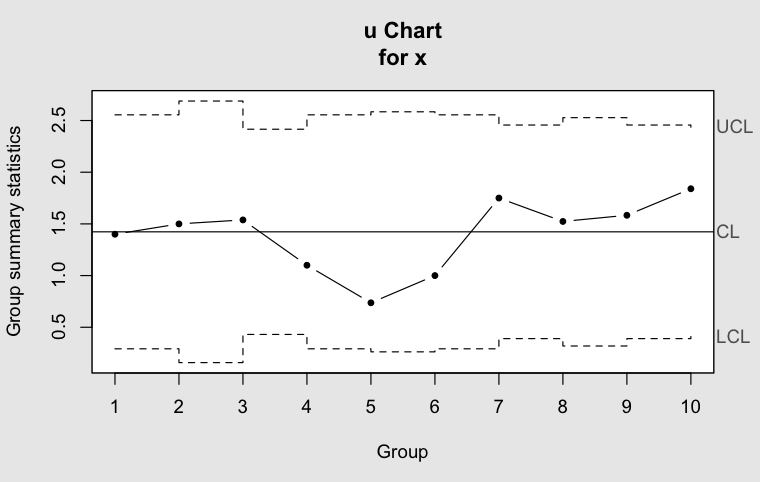
\includegraphics[width=1.0\linewidth]{u-chart-R}
\end{figure}
\end{frame}
%============================================================ %
\end{document}